%
%

%%-----------------------------------------------------
%%-----------------------------------------------------
\section{En las nubes}

%%-----------------------------------------------------
\begin{frame}
\frametitle{OpenStack}

\begin{columns}[T]
\begin{column}{.38\textwidth}

\includegraphics[width=6.5cm]{figs/openstack-logo}

\begin{flushright}
\url{http://openstack.org}
\end{flushright}

\end{column}%
\hfill%
\begin{column}{.60\textwidth}
{\Large
\begin{itemize}
\item Plataforma para la computación en nube
\item Software libre
\item Tecnología básica: \\
  Python / Django
\item Gestión vía línea de comandos, \\
  API REST, dashboard
\item Inicio: 2010 \\
  (NASA, Rackspace)
\item Gestionado por la \\
  OpenStack Foundation
\end{itemize}
}
\end{column}%
\end{columns}

\end{frame}

%%-----------------------------------------------------
\begin{frame}
\frametitle{Principales components}

\begin{columns}[T]
\begin{column}{.45\textwidth}
{\Large
\begin{itemize}
\item Computación
\item Almacenamiento de objetos
\item Almacenamiento de bloques
\item Red
\item Dashboard
\end{itemize}
}
\end{column}%
\hfill%
\begin{column}{.45\textwidth}
{\Large
\begin{itemize}
\item Servicio de identidades
\item Servicio de imágenes
\item Telemetría
\item Orquestación
\item Base de datos
\item Metal desnudo
\end{itemize}
}
\end{column}%
\end{columns}

\end{frame}

%%-----------------------------------------------------
\begin{frame}
\frametitle{Horizon: el dashboard}

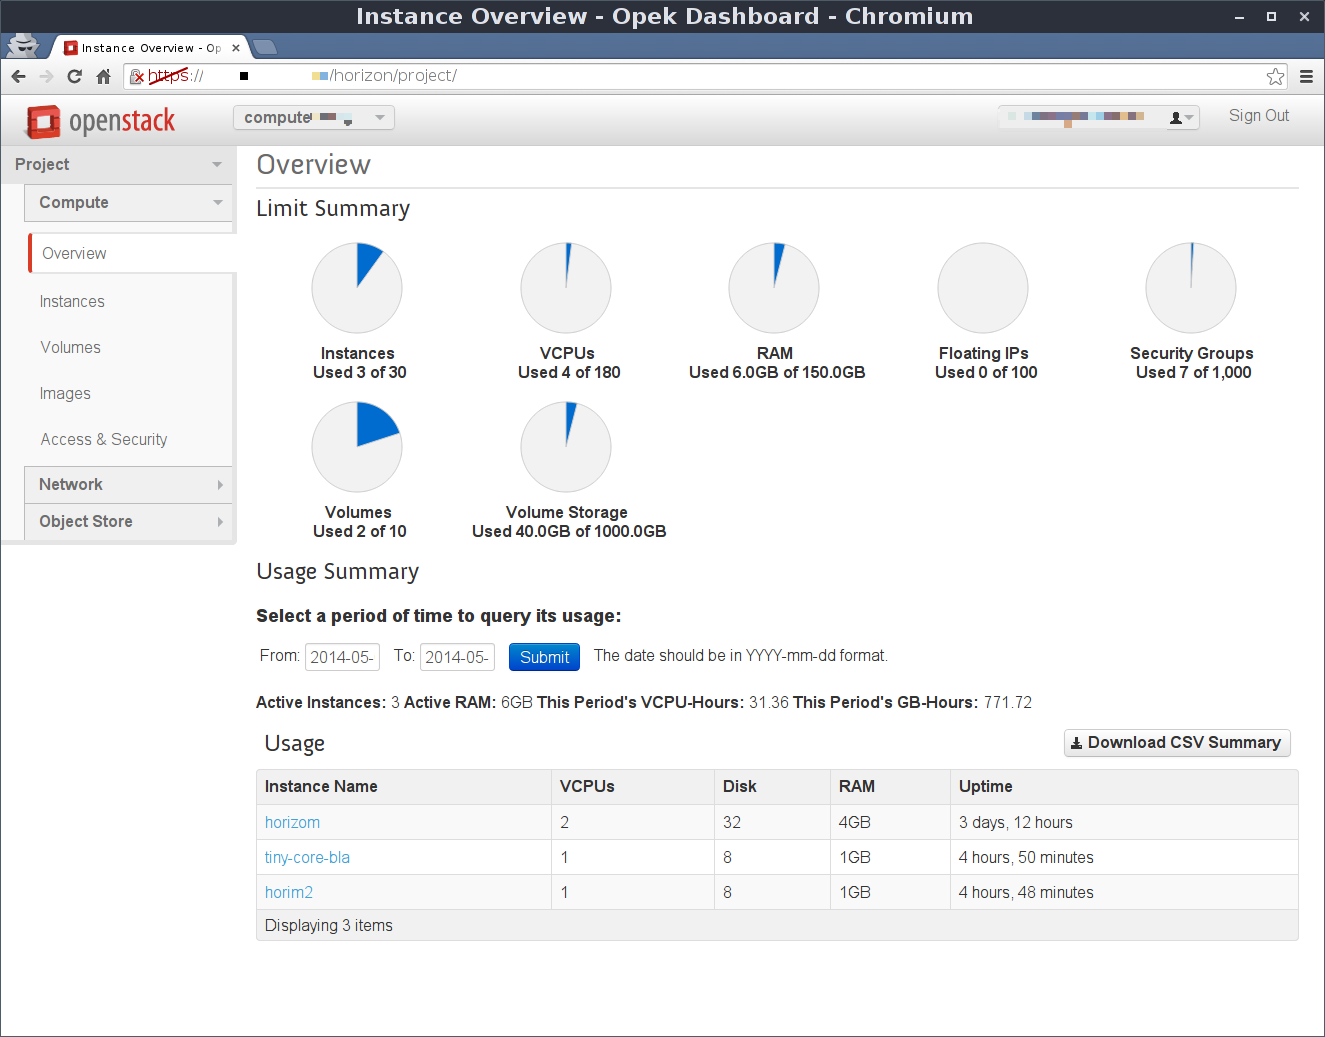
\includegraphics[height=7cm]{figs/openstack-screenshot}

\begin{flushright}
\url{https://www.youtube.com/watch?v=TgPTjrf1y0A}
\end{flushright}

\end{frame}

%%-----------------------------------------------------
\begin{frame}
\frametitle{Las empresas}

\begin{columns}[T]
\begin{column}{.55\textwidth}
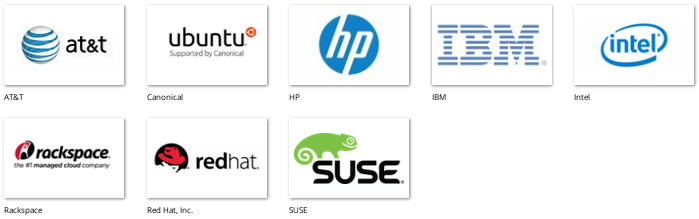
\includegraphics[width=6.5cm]{figs/openstack-platinum}\\
\vspace{1cm}
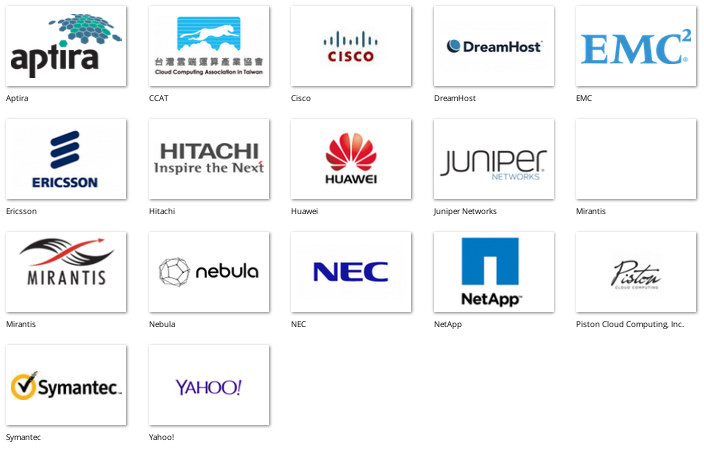
\includegraphics[width=6.5cm]{figs/openstack-gold}\\
\end{column}%
\hfill%
\begin{column}{.41\textwidth}
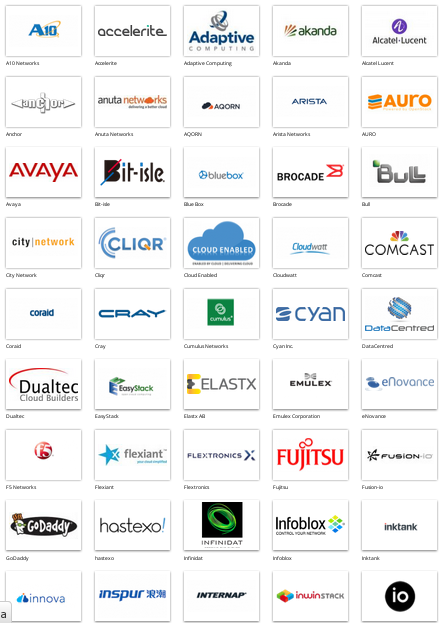
\includegraphics[width=4.5cm]{figs/openstack-silver}
\end{column}%
\end{columns}

\end{frame}





